%----------------------------------------------------------------------------------------
%	CHAPTER
%----------------------------------------------------------------------------------------

\chapter{필수 파이썬 라이브러리}

지금부터 사용할 아이브러리와 과학계산용 파이썬 환경에 익숙하지 않은 사용자를 위해 간단히 라이브러리를 소개한다.

\section{Numpy}\index{Numpy}

NumPy(http://numpy.org)는 Numerical Python의 줄임말로, 과학계산용 파운데이션 패키지이다. 다음은 NumPy의 기능이다.


\begin{itemize}
	\item{빠르고 효율적인 다차원 배열 객체ndarray}
	\item{배열 원소를 다루거나 배열 간의 수학 계산을 수행하는 함수}
	\item{디스크로부터 배열 기반의 데이터를 읽거나 쓸 수 있는 도구}
	\item{선형대수 계산, 푸리에 변환, 난수 발생기}
	\item{파이썬과 C, C++ 그리고 포트란 코드를 통합하는 도구}
\end{itemize}


NumPy는 파이썬에 빠른 배열 처리 기능을 제공하며, 데이터 분석에서는 알고리즘에 사용할 데이터 컨테이너의 역할을 한다. 수이데이터라면 NumPy 배열은 파이선 기본 자료 구조보다 훨씬 효율적인 방법으로 데이터를 저장하고 다룰 수 있다. 또한 C나 포트란 같은 저수준 언어로 이루어진 라이브러리는 NumPy 배열에 저장된 데이터를 복사하지 않고 사용할 수 있다. 


\section{Matplotlib}\index{Theorems}

https://matplotlib.org/

matplotlib \은 그래프나 2차원 데어터 시각화를 생성하는 유명한 파이썬 라이브러리다. Jhn D. Hunter \가 만들었고, 지금은 만은 배발 팀이 유지하고 있다. 출판물에 필요한 그래프를 만드는 데 맞춰졌으며 IPython에 통합되어 있어 편리하게 데이터를 살펴보고 그래프를 만들수 있다. IPython에서 matplotlib \로 생성한 그래프는 그래프 창에 있는 툴바로 특정 부분을 확대하거나 그래프의 여기저기를 인터랙트브하게 살펴볼 수 있다.


\section{matplotlib basemap toolkit}\index{basemap}

The matplotlib basemap toolkit is a library for plotting 2D data on maps in Python. It is similar in functionality to the matlab mapping toolbox, the IDL mapping facilities, GrADS, or the Generic Mapping Tools. PyNGL and CDAT are other libraries that provide similar capabilities in Python.

Basemap does not do any plotting on it’s own, but provides the facilities to transform coordinates to one of 25 different map projections (using the PROJ.4 C library). Matplotlib is then used to plot contours, images, vectors, lines or points in the transformed coordinates. Shoreline, river and political boundary datasets (from Generic Mapping Tools) are provided, along with methods for plotting them. The GEOS library is used internally to clip the coastline and polticial boundary features to the desired map projection region.

Basemap is geared toward the needs of earth scientists, particularly oceanographers and meteorologists. Jeff Whitaker originally wrote Basemap to help in his research (climate and weather forecasting), since at the time CDAT was the only other tool in python for plotting data on map projections. Over the years, the capabilities of Basemap have evolved as scientists in other disciplines (such as biology, geology and geophysics) requested and contributed new features.


\subsection{지도 그리기}\index{지도 그리기}

Figure \ref{fig:mapofkorea01} \과 같은 지도를 그려보자.
\begin{figure}[h]
	\centering
	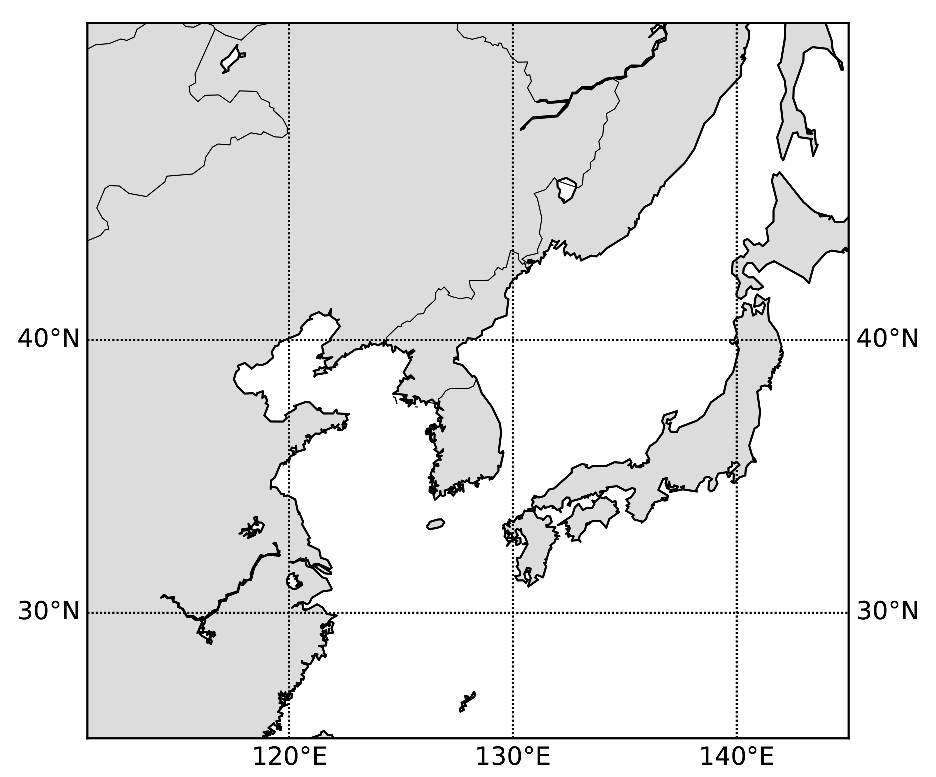
\includegraphics[width=0.7\linewidth]{MapOfKorea01}
	\caption{한반도 주변 지도(메르카토르도법)}
	\label{fig:mapofkorea01}
\end{figure}



\begin{code}[한반도 주변 지도(메르카토르도법)]
%	\begin{align}
	\begin{lstlisting}

#python 
from mpl_toolkits.basemap import Basemap
import matplotlib.pyplot as plt
import numpy as np

# create new figure, axes instances.
fig = plt.figure()
ax = fig.add_axes([0.1,0.1,0.8,0.8])

#loglat = [west,south,east,north]
loglat = [111,25,145,50]
clog = (loglat[2]+loglat[0]) / 2
clat = (loglat[3]+loglat[1]) / 2

#map projection.
m = Basemap(llcrnrlon=loglat[0],llcrnrlat=loglat[1],\
	urcrnrlon=loglat[2],urcrnrlat=loglat[3],\
	rsphere=(6378137.00,6356752.3142),\
	resolution='l',projection='merc',\
	lon_0=clog,lat_0=clat,lat_ts=20.)

m.drawcoastlines()
m.drawcountries()
m.fillcontinents()

# draw parallels
m.drawparallels(np.arange(10,90,10),labels=[1,1,0,1])
# draw meridians
m.drawmeridians(np.arange(-180,180,10),labels=[1,1,0,1])

plt.show()

		\end{lstlisting}
%		\end{align}
\end{code}

\subsection{일기도 모양의 지도 그리기}\index{일기도 모양의 지도 그리기}

Figure \ref{fig:surf201707021} \은 기상청(http://www.kma.go.kr/weather/images/analysischart.jsp)에서 제공하는 지상일기도이다. 

\begin{figure}[h]
	\centering
	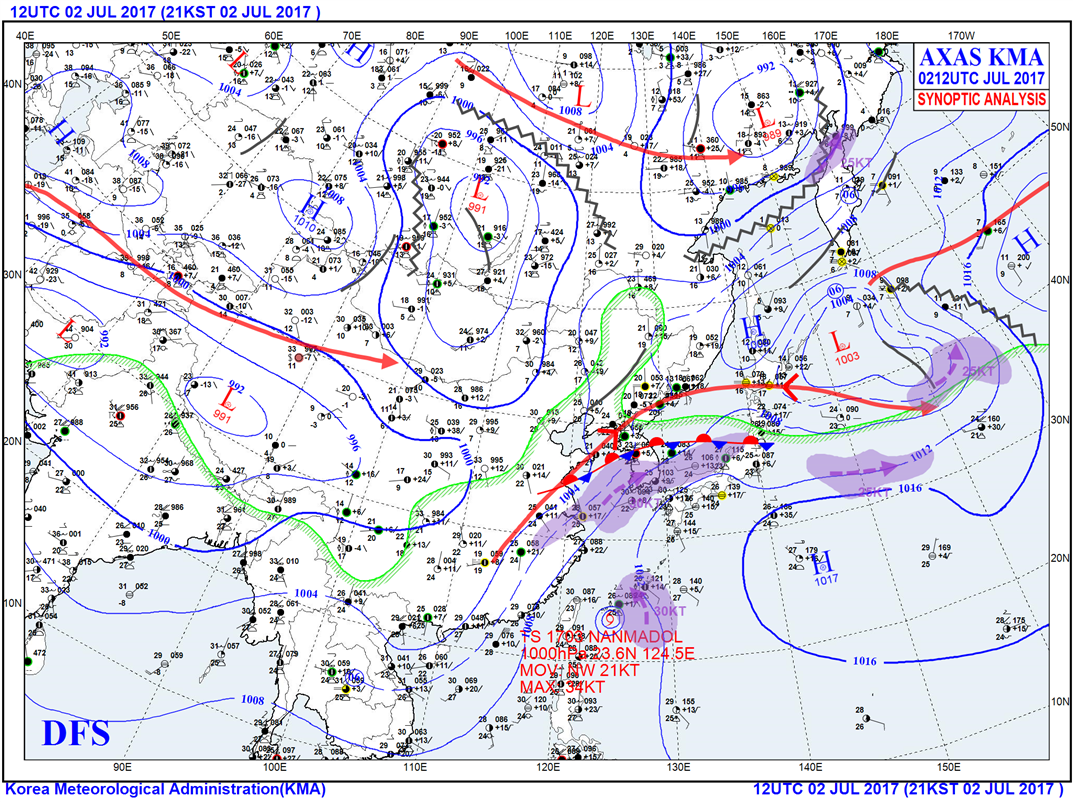
\includegraphics[width=0.8\linewidth]{surf_2017070212}
	\caption{기상청 지상일기도}
	\label{fig:surf2017070212}
\end{figure}

이와 비슷한 지도를 그리는 코드틑 다음과 같다.

\begin{code}[기상청 일기도모양 백지도]
	%	\begin{align}
	\begin{lstlisting}
	
from mpl_toolkits.basemap import Basemap
#python 
import matplotlib.pyplot as plt
import numpy as np

# create new figure, axes instances.
fig=plt.figure()
ax=fig.add_axes([0.1,0.1,0.8,0.8])

#loglat = [west,south,east,north]
loglat = [90,0,180,62]
clog = (loglat[2]+loglat[0])/2
clat = (loglat[3]+loglat[1])/2

# map projection.
m = Basemap(llcrnrlon=loglat[0],llcrnrlat=loglat[1],\
	urcrnrlon=loglat[2],urcrnrlat=loglat[3],\
	resolution='l',projection='aea',lon_0=clog,lat_0=clat)

m.drawcoastlines()
m.drawcountries()
m.fillcontinents()

# draw parallels
m.drawparallels(np.arange(0,90,10),labels=[1,1,0,0])
# draw meridians
m.drawmeridians(np.arange(-180,180,20),labels=[0,0,1,0])
m.drawmeridians(np.arange(-180,180,10),labels=[0,0,0,1])

plt.show()	
	\end{lstlisting}
	%		\end{align}
\end{code}

그 결과이다. 

\begin{figure}[h]
	\centering
	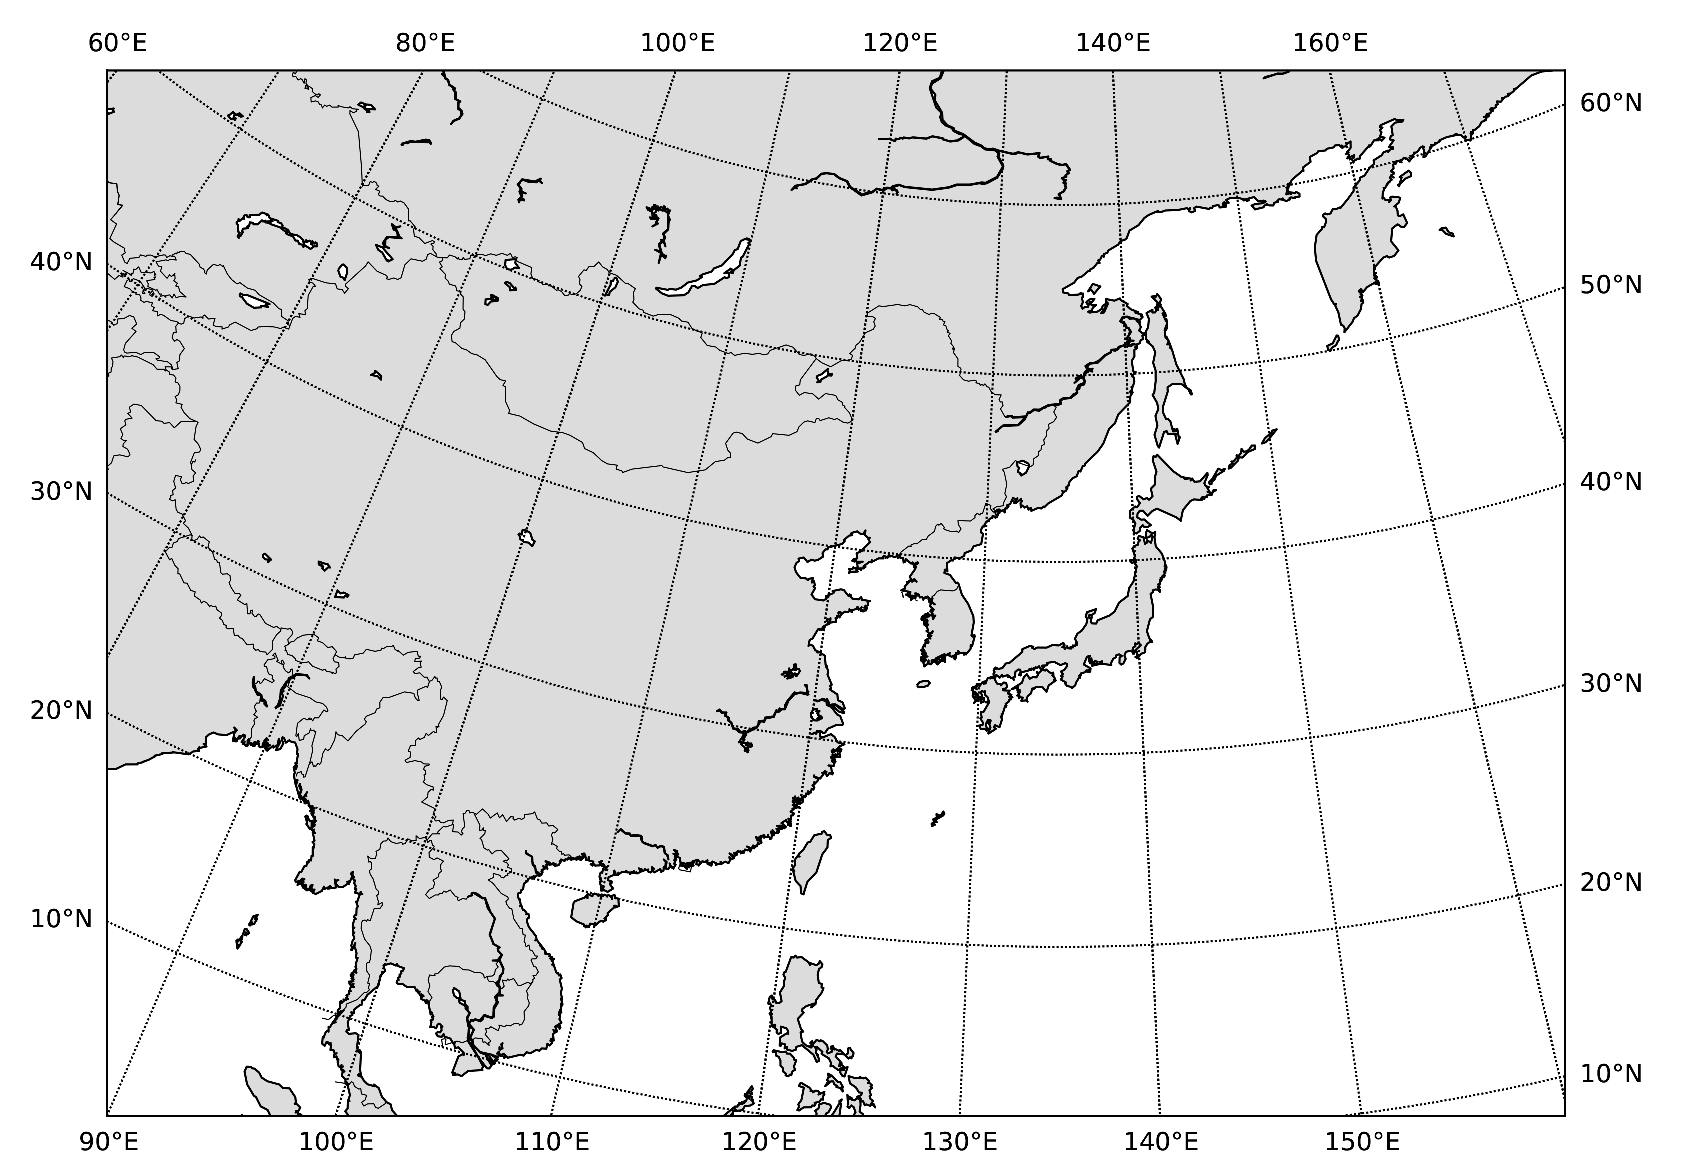
\includegraphics[width=0.8\linewidth]{weathermap01}
	\caption{기상청 일기도모양 백지도}
	\label{fig:weathermap01}
\end{figure}